%%%%%%%%%%%%%%%%%%%%%%%%%%%%%%%%%%%
%% Appendix
%%%%%%%%%%%%%%%%%%%%%%%%%%%%%%%%%%%
In this appendix we succinctly describe the contents of each file. We
include in 
Figure~\ref{fig:deps}  a dependency graph of our formalization. The
theories on a grayish background are directly from Paulson; we
highlight with blue/cyan those of Paulson that we modified. We
have developed from scratch the rest, in white.

\begin{description}[itemsep=1.5pt]
\item[\texttt{Nat\_Miscellanea}]Miscellaneous results for naturals, mostly
  needed for renamings.
\item[\texttt{Renaming}] Renaming of internalized formulas, see
  Section \ref{sec:renaming}.
\item[\texttt{Pointed\_DC}] A pointed version of the Principle of
  Dependent Choices.
\item[\texttt{Recursion\_Thms}] Enhancements about recursively defined
%\newpage
  functions.
\item[\texttt{Forcing\_Notions}] Definition of Posets with maximal
  element, filters, dense sets. Proof of the Rasiowa-Sikorski Lemma.
\item[\texttt{Forcing\_Data}] Definition of the locales:
  \begin{inlinelist}
  \item \texttt{M\_ZF} satisfaction of axioms; and 
  \item \texttt{forcing\_data} extending the previous one with
    \texttt{forcing\_notion}, transitivity, and being countable.
  \end{inlinelist}
\item[\texttt{Interface}] Instantiation of locales \texttt{M\_trivial}
  and \texttt{M\_basic} for every instance of \texttt{Forcing\_Data}.
\item[\texttt{Names}] Definitions of $\chk$, $\val$, and the generic
  extension. Various results about them.
\item[\texttt{Forcing\_Theorems}] Specification of fundamental
  theorems of forcing, see Section~\ref{sec:forcing}.
\item[\texttt{*\_Axiom}] Proof of the satisfaction of the
  corresponding axiom in the generic extension.
\end{description}
%
\begin{figure*}[!b]
  \begin{center}
    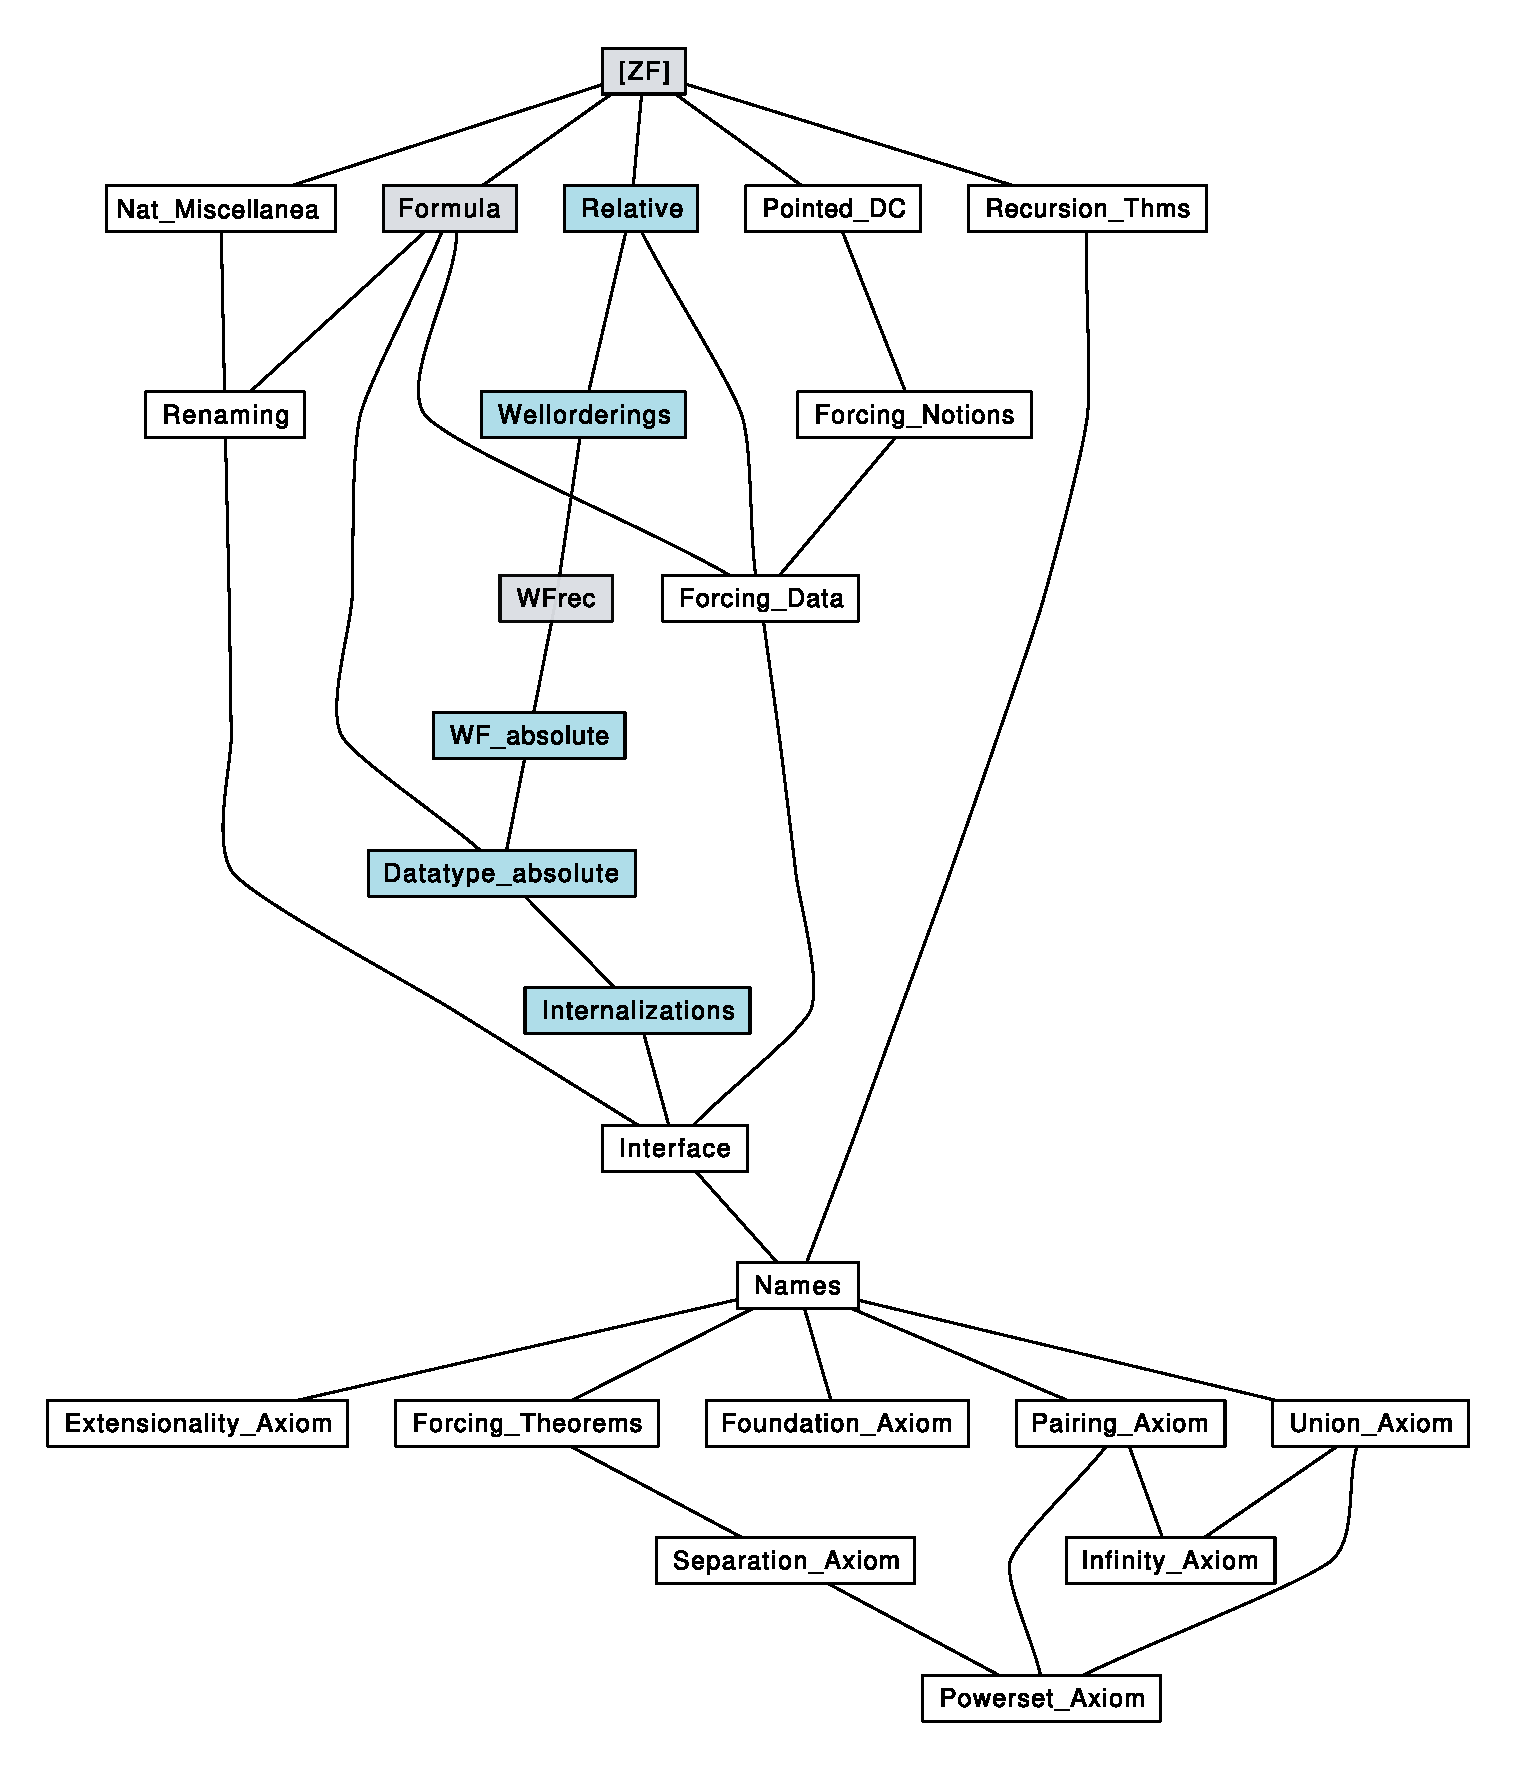
\includegraphics[height=14cm]{session_graph_colored.pdf}
  \end{center}
  \caption{Dependency graph of the \isatt{Separation} session.}
  \label{fig:deps}
\end{figure*}

%%% Local Variables: 
%%% mode: latex
%%% TeX-master: "Separation_In_MG"
%%% ispell-local-dictionary: "american"
%%% End: 
